\documentclass [8pt,fleqn]{article}

\usepackage{color}
\usepackage{amssymb}
\usepackage[font={small,it}]{caption}
\usepackage{bm}
\usepackage{draftwatermark}
\usepackage{epsf,graphicx}
\usepackage{psfrag}
\usepackage{textcomp}
\usepackage{float}
\usepackage{amsmath}
\usepackage{siunitx}
\usepackage[mathscr]{euscript}
\usepackage{color}
\usepackage{verbatim}
\usepackage{authblk}
\usepackage{lineno}


\SetWatermarkText{Draft}
\SetWatermarkScale{5}

\usepackage[a4paper,bindingoffset=0.2in,%
            left=1in,right=1in,top=1in,bottom=1in,%
            footskip=.25in]{geometry}

\makeatletter
\g@addto@macro\@floatboxreset\centering
\makeatother
            

%\topmargin     -0.60in  % (adjusted for printer bias) 
%\headheight      .00in  % (no headers) 
%\headsep         .50in  % (top margin + headers + skip) 
\textheight     9.50in  % (instructions: 9 1/8'' min, 9 7/16'' max) 
%\textwidth      7.00in  % 2*3.33 + .33 = 6.99 
%\oddsidemargin  0.3125in  % (subtracted 1inch bias) 
%\evensidemargin 0.3125in  
\parindent .0in 
\parskip 10pt 

\newcommand*{\matminus}{%
  \leavevmode
  \hphantom{0}%
  \llap{%
    \settowidth{\dimen0 }{$0$}%
    \resizebox{1.1\dimen0 }{\height}{$-$}%
  }%
}

\renewcommand*{\thefootnote}{\fnsymbol{footnote}}
\newcommand{\angstrom}{\textup{\AA}}


\font \bigtenrm=cmmi10 scaled\magstep2 
\def \be {\begin{equation}} 
\def \ee {\end{equation}} 
\def \beq {\begin{eqnarray}} 
\def \eeq {\end{eqnarray}} 


\title{Observation of wide-angle correlated X-ray scattering of nanoparticles agrees with atomic twinning model}

\author{Derek Mendez}
\author[1]{Herschel Watkins}
\author[1]{Kevin Raines}
\author[2]{ Thomas J. Lane}
\author[1]{Gundolf Schenk}
\author[4]{Kensuke Tono}
\author[4]{Yasumasa Joti}
\author[3]{Makina Yabashi}
\author[2]{Daniel Ratner}
\author[1,2]{Sebastian Doniach}

\affil [1]{Stanford University Department of Applied Physics, Stanford, CA 94305}
\affil [2]{SLAC National Accelerator Laboratory, Menlo Park, CA 94025}
\affil [3]{RIKEN SPring-8 Center, Kouto 1-1-1, Sayo, Hyogo 679-5148, Japan}
\affil [4]{Japan Synchrotron Radiation Research Institute (JASRI), Kouto 1-1-1, Sayo, Hyogo 679-5198, Japan}

\renewcommand\Authands{ and }

\begin{document}
\maketitle
\delimitershortfall=-1pt

\begin{center}
\section*{Abstract}
\end{center}
We report on measurement of angular intensity correlations resulting from snapshot exposures of gold nanoparticles recorded at the Spring-8 Angstrom Compact Free Electron Laser facility (SACLA). Each exposure was a snapshot of X gold nanoparticles (each Y nm in size) suspended freely with random orientations. From analysis of the intrinsic uncorrelated background we evaluated the number of exposures needed to assess the significance of the observed CXS signal. By looking at wide angles, we were able to compare the CXS signal to an atomic twinning model. We show that the data may be represented in terms of CXS from a decahedral twinning model.

%Twinning was observed from isotropic solution exposures recorded at the SPring-8 Angstrom Compact Free Electron Laser facility (SACLA).  Each exposure was a snapshot of roughly 90,000 gold particles (each 60 nanometers across) suspended freely with random orientations. Twinning, which is readily observed using electron microscopy techniques, can go unnoticed in conventional X-ray scattering measurements which require long exposures that average away azimuthal variations (e.g. wide angle X-ray scattering / WAXS ). By using correlated X-ray scattering (CXS) analysis, we resolved a signal indicative of a basic twinning structure common to the nanoparticles. Our data also agree with a more complex decahedral twinning model. We hope this experiment sheds a new light on CXS as a technique for resolving local structural details from solution measurements.

\section*{Acknowledgements}
The XFEL experiments were performed at the BL3 of SACLA with the approval of the Japan Synchrotron Radiation Research Institute (JASRI) (Proposal No. 2013B8009 )

\section{Introduction}
Correlated X-ray scattering (CXS) is an emerging field which involves recording many snapshot exposures of an ensemble of randomly oriented mono-dispersed molecules or particles, and employing photon intensity correlation analysis to recover the average internal structure of the objects in the random ensemble \cite{Kam77}. CXS has potential to reveal the structural properties of proteins and soft matter without the use of crystallization \cite{SaldinBeyond, SaldinIsolated, SaldinTowards, PandeDeduce, GundDNA}. An obvious precursor to the study of soft matter CXS is that of nanoparticles (NPs), due to their typically large scattering cross sections. Here we will discuss an experiment involving three-dimensional NP suspensions. NP suspensions are used in chemical catalysis, and their chemical properties are directly related to  the overall shape and atomic structure of the NPs themselves \cite{YacaShapeDepend, ShapeDepend2, ShapeDepend3}. As such, there is a need for structural characterization methods. Past work describing the thermodynamics and kinetics of NP growth and formation \cite{InoStability, MarksWulff, HowieMarks, MarksSurf, KinTherm} has revealed that smaller NPs tend to form complicated twinning structures, e.g. decahedral and icosahedral twins \cite{HeinemannStruct, YacaStruct, NPseeds, YangGeom, YangSymm, DaiShapes}. Previously, twinning has been observed using electron microscopy and tomography \cite{MarksGoldSilv, YacaEM, 3Dimg}, where one images single NP projections. On the other hand, conventional powder X-ray diffraction measurements, used widely in industry to characterize ensembles of NPs, are isotropic averages and don't show signs of twinning. In what follows we will show how CXS can reveal twinning from many snapshot exposures of a solution of gold NPs. Further, we will show how the CXS signal scales with the number of correlated snapshots.

\begin{figure}[H]
\begin{center}
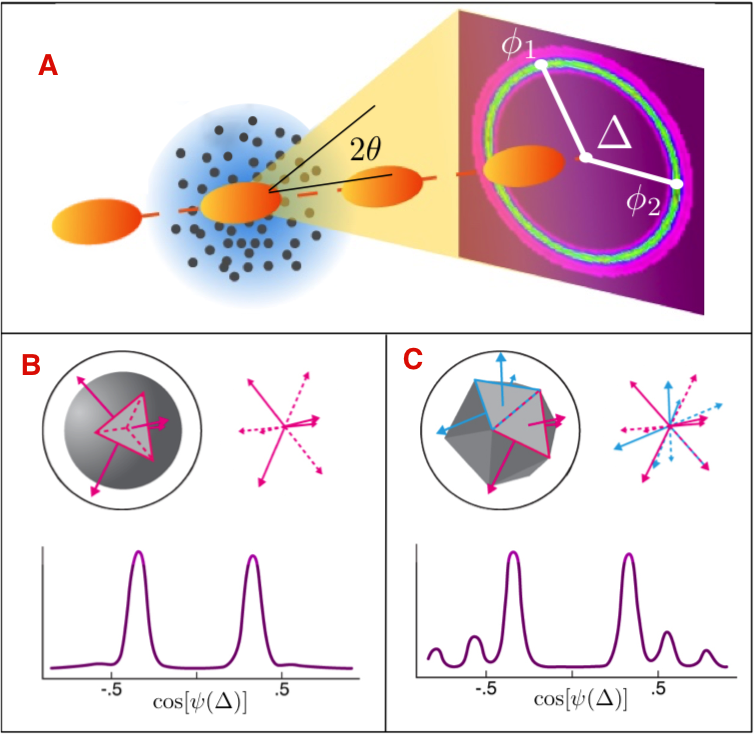
\includegraphics[keepaspectratio, scale=0.9]{./fig1_new_version2.png}
\end{center}
\caption{Distinguishing twinned NPs from single domain NPs using CXS. \textbf{A)} A free electron laser pulse (orange) exposes a collection of nanoparticles (black). Individual NPs scatter photons into specific angles (e.g. $\phi_1$, $\phi_2$, separated by $\Delta$). The total scatter from the NP collection results in a powder diffraction ring ($\{111\}$ Bragg ring highlighted in green), which by itself gives no indication of twinning. \textbf{B)} A bulk face-centered-cubic NP with a spherical boundary and the corresponding $\{111\}$ CXS signal. The expanding planes are outlined in pink, showing a regular tetrahedron. The plotted correlation signal has two pronounced peaks at $\pm (1/3)$, corresponding to the $70.5^{\circ}$ and $109.5^{\circ}$ angles between the planes of a regular tetrahedron. This would be the expected $\{111\}$ correlation from any bulk face-centered-cubic (FCC) crystal. \textbf{C)} An icosahedral twinned FCC nanoparticle and the corresponding $\{111\}$ CXS signal due to a nearest-neighbor twinned unit (highlighted in blue and pink). The icosahedron is formed by 10 nearest-neighbor twinned units - each unit consisting of two regular FCC tetrahedrons related by a reflection about the common plane (referred to as the twin boundary). The CXS signal shows pronounced peaks at $\pm (1/3), \pm (5/9), \pm (7/9)$, which correspond to the angles between all pairs of $\{111\}$ planes in a nearest-neighbor twin unit. The increased complexity of the CXS signal is illustrated by the cluster of blue and pink Bragg vectors. Artwork courtesy of Gregory M.~Stewart (SLAC).}
\label{fig:contrast}
\end{figure}

\section{Background}
CXS has been extensively explored as a tool to investigate two-dimensional systems \cite{KurtaMembrane, SchroerFilms, Lehm2D, Kurta2D, Pedrini2D, Saldin2D}, however in three-dimensioal systems, the information content accessible by CXS techniques decreases \cite{ElserStrat}. If one or few three-dimensional objects are exposed during each snapshot, then one can use symmetry arguments to recover structural information content \cite{KamMicroG, SaldinTricks, Liu3D, ChenDumbbell, StarodubSingle, SaldinSingle}. When the number of exposed three-dimensional objects increases, one can still use the correlated intensities to infer local structural characteristics \cite{Woch, AltarelliGen, Oxy, MalmerbergOp}, resolve structural changes \cite{PandeTime}, and possibly even refine atomic models in an iterative procedure \cite{HaiguangZern}. In this paper report on CXS as a tool to investigate a three-dimensional ensemble of gold NPs, where each snapshot is composed of many NPs. First we qualitatively describe the physics of CXS for NP ensembles.

An object in solution exposed to sufficient X-ray flux over a short time interval can scatter photons into at least two directions, $\bm q_1$ and $\bm q_2$. While the orientation of this object can be random, the angle defined by $\bm q_1$ and $\bm q_2$ 

\be \label{cpsi}
\cos (\psi) = (\bm q_1 \cdot \bm q_2)/(q_1 \, q_2 )
\ee

is not; it is biased by the object's internal atomic structure. A crystalline NP scatters photons into discrete Bragg vectors $\bm q_{hkl}$. We define a detector who's pixels correspond to a set of Bragg vectors $\{\bm q\}$. Let $\omega$ be a triple of Euler angles defining an NP orientation relative to some axis (e.g. that of an X-ray beam). An NP at orientation $\omega$ can scatter photons into the detector provided

\be \label{condition}
\hat{\bm R}_\omega \cdot \bm q_{hkl} \in \{\bm q\}
\ee

where $\hat{\bm R}_\omega$ is an operator which rotates the NP from some pre-defined arbitrary orientation into $\omega$. We assume a small fraction of NPs in solution are oriented such that condition (\ref{condition}) is met for two Bragg vectors, $\bm q_{hkl}$ and $\bm q_{h'k'l'}$. When one NP is oriented as such, and if it scatters photons into both $\bm q_{hkl}$ and $\bm q_{h'k'l'}$, then these photons are said to be correlated. This double Bragg scattering produces angular intensity correlations between pairs of Bragg vectors in $\{\bm q\}$ whose angular separation $\psi$ is defined by

\be \label{hklcorr}
\cos(\psi_{hkl,h'k'l'}) =\frac{ \bm q_{hkl} \cdot \bm q_{h'k'l'} } {q_{hkl}\, q_{h'k'l'}} 
\ee

The angle $\psi_{hkl,h'k'l'}$ is also the interplanar angle between crystallographic planes $hkl$ and $h'k'l'$. Typically, the pixels $\{\bm q\}$ are arranged on a planar detector, assumed perpendicular to the forward X-ray beam (Figure \ref{fig:contrast}A). With such a setup, it is often convenient to express correlations in terms of the azimuthal angle $\phi$ which spans the detector plane $(0 \le \phi \le 2\pi)$. The azimuthal degree of separation, $\Delta = \phi_1  - \phi_2$, between any 2 pixels on the detector can be expressed in terms of (\ref{cpsi}) via

\be \label{project}
\cos(\psi) = \cos( \Delta )\cos( \theta_1)\cos(\theta_2) + \sin(\theta_1)\sin(\theta_2)
\ee

(Figure \ref{fig:contrast} B,C) where $\theta$ is half the Bragg angle for elastically scattered photons at wavelength $\lambda$, defined by

\be
\theta  = \arcsin \big( \,\frac{ \lambda\,q  }{ 4\pi }\, \big )
\ee

(Figure \ref{fig:contrast} A). Geometrically, $\psi$ has a maximum when $\Delta=\pi$, hence

\be \label{psimax}
\cos(\psi_{max}) = - \cos( \theta_1)\cos(\theta_2) + \sin(\theta_1)\sin(\theta_2)
\ee

which sets a bound on the correlation angles (\ref{cpsi}) that can measured in a given experiment. Note, at small scattering angles, $\psi \rightarrow \Delta$. The large majority of CXS experimental work to date has been conducted in this small angle limit.

In a typical exposure, most NPs will not scatter into the detector, hence a small fraction will be oriented such that they scatter into multiple detectable directions \cite{Observ} . Therefore, the average exposure comprises a large fraction of randomly scattered and uncorrelated photons (owing to the orientation randomness in a solution). As such, the correlation signal-to-noise is much less than unity for a single exposure, which has been shown to scale as the square root of the number of averaged exposures, $N_s$ \cite{Kirian}. We consider an exposure to be a snapshot, meaning the NPs should not be moving significantly throughout the exposure duration. This is guarantteed by the femto-second timescale pulses of the SACLA facility \cite{ImagingPotential}. CXS can also be conducted at synchrotron radiation facilities, provided that the sample is prepared in an anti-freeze suspension, and that it is cooled during exposure to prevent motion of the particles \cite{KamSynch,Observ}. 

\section{Theory}
Each gold NP has a well-defined face-centered-cubic (FCC) lattice structure. This paper only discusses correlations arising from the $\{111\}$ family of planes. There are 4 distinct $\{111\}$ planes: $111$,$11\bar 1$,$\bar 1 1\bar 1$,$1\bar 1 \bar 1$, and the mirror-symmetric planes, $\bar 1\bar 1\bar 1$,$\bar 1\bar 1 1$,$1 \bar 11$,$\bar 1 1 1$.  Photons scattered from these crystallographic planes from an ensemble of randomly oriented NPs will form a Bragg ring at  $q_{111} = 2\pi / d_{111} $ where $d_{111}$ is the inter-planar spacing. Let 

\be
\bm Q_{111} = \big \{\bm q_{111}, \bm q_{11\bar 1},\bm q_{\bar 1 1\bar 1},\bm q_{1\bar 1 \bar 1},\bm q_{\bar 1\bar 1\bar 1},\bm q_{\bar 1\bar 1 1},\bm q_{1 \bar 11},\bm q_{\bar 1 1 1} \big\}
\ee

be the set of $\{111\}$ Bragg vectors. We let 

\be
\mathbb F \big[ \bm q_1, \bm q_2\big] =  (\bm q_1 \cdot \bm q_2)/(q_1 \, q_2 ) = \cos( \psi )
\ee

be the operation which takes a pair of vectors, and returns the cosine of the angle between them. With this we can express analytically which angles $\psi$ give rise to correlations by forming the sequence

\be \label{psiset}
\bm \Psi_{111} = \left \{ \mathbb F\big[  \bm q_1, \bm q_2 \big ] \, \,\forall \, \, (\bm q_1, \bm q_2 \ne \bm q_1) \in \bm Q_{111}\,  \big | \,  \arccos \bigg( \mathbb F \big [  \bm q_1, \bm q_2\big ] \bigg )  \, \le \,  2\theta_{111}   \right \}
\ee 

where we made use of (\ref{psimax}). Note, $\mathbb F\big [ \bm q, -\bm q \big ]  = -1$ corresponding to a correlation angle of $\pi$ is not included in the sequence as this angle is not measurable using conventional flat detectors. Evaluating the sequence $(\ref{psiset})$ we find it only contains values $\pm (1/3)$. This is in agreement with the peaks shown in  Figure \ref{fig:contrast}B.

The above CXS analysis assumes that each gold NP is a single FCC domain. It is well known that smaller FCC NPs are not single crystal domains. Instead, they tend to form complicated twinning structures composed of many tetrahedral sub-units \cite{MarksGoldSilv}. The reciprocal space of these structures is more complex than that of a single domain NP, but this complexity is hidden in standard powder diffraction images; the twins all scatter into the same Bragg rings. CXS, however, is sensitive to twinned NPs. Consider the following simple model for two FCC tetrahedrons joined by a twinning plane. Let each face of the tetrahedrons be a $\{111\}$ plane. When joined, the tetrahedrons will have 1 plane in common, referred to as the twinning plane. The twins' atomic coordinates are related to one another by a reflection about this plane. We refer to this twinned structure as a nearest-neighbor twin (NNT). Larger structures, e.g. decahedrons and icosahedrons, can be assembled with NNTs (Figure \ref{fig:contrast}c). We call the twins ``\,twin$_A$" and ``\,twin$_B$".  In this simple model, twin$_A$ is oriented relative to twin$_B$ via a rotation of $\pi$ about its $(111)$ direction. This operation is given by the matrix

\be \label{twinmat}
\mathbf T = \begin{bmatrix}
       \frac{-1}{3} & \frac{2}{3} & \frac{2}{3}           \\[0.3em]
       \frac{2}{3} & \frac{\matminus 1}{3}           & \frac{2}{3} \\[0.3em]
       \frac{2}{3}           & \frac{2}{3} & \frac{-1}{3}
     \end{bmatrix}
\ee

During an exposure, photons can scatter from each twin into separate, but correlated, Bragg vectors. We refer to these correlations as inter-twin correlations. Let us define the set of Bragg vectors for the NNT model as 

\be
\bm Q^{A,B}_{111}\,\, =\,\, \bm Q_{111} \, \cup \, \big \{  \mathbf T  \cdot \bm q \, \forall \, \bm q \in \bm Q_{111} \big \}
\ee

We can now predict where NNTs will give correlations using this new set of vectors: 

\be \label{psisetab}
\bm \Psi^{A,B}_{111} = \left \{ \mathbb F\big[ \bm q_1, \bm q_2 \big ] \, \forall \, (\bm q_1, \bm q_2 \ne \bm q_1) \in \bm Q^{A,B}_{111}\, \big | \,  \arccos \bigg(  \mathbb F \big[  \bm q_1, \bm q_2 \big ] \bigg ) \, \le \,  2\theta_{111}     \right \}
\ee

For experiments with sufficiently large $2\theta_{111}$, (\ref{psisetab}) will contain only values $\pm (1/3), \pm (5/9), \pm(7/9)$ (Figure \ref{fig:contrast}C). 

Note we reached these conclusions by considering the atomic structure of a single NP; the information content of CXS depends solely on the scattering factor of the individual particle in solution.

Depending on the growth process, gold NPs have been observed to grow into many complicated twinned shapes, referred to as multiply-twinned particles (MTPs). In an MTP, there are additional correlations which can arise due to next-nearest-neighbor twins and so-forth. As the particles get more complex, so does the CXS. One can imagine using CXS to distinguish various shapes of nanoparticles in solution, though such analysis is beyond the scope of this report. 

\section{Experiment}
Here we report on the successful measurement of CXS for gold NPs at the SACLA beam facility in Japan. Sixty-nanometer gold NPs were purchased from Nanopartz Inc. and suspended in LCP (lipid cubic phase) at a concentration of 40 mg/ml. The viscous solution was injected into the beam as a constant stream using a  hamilton 7780 syringe needle with inner diameter \SI{130}{\micro \meter}. The SACLA beam was focused down to a roughly \SI{1.5x2.4}{ \micro \meter } spot size, and from these numbers we estimate roughly $9 \cdot 10^4$ particles in the beam during each exposure. 

The beam repetition rate was 30 Hz. The pulses were measured using an MPCCD 8-panel detector in a wide-angle setup, with a beam energy of \SI{8.6}{\kilo \electronvolt} and a maximum scattering angle of $3.4 \, \angstrom^{-1}$.  With this setup we acquired roughly $5 \cdot 10^5$ snapshot exposures of gold NPs. For the analysis we worked solely with the $\{111\}$ Bragg ring.

The goal of the analysis was to determine the angles $\psi$ which show angular intensity correlations at the $\{111\}$ Bragg ring, and to compare the results with the values in (\ref{psiset}) and (\ref{psisetab}).

\section{Results}
Conventional CXS analysis involves computation of angular correlations in the azimuthal component of the planar detector

\be \label{cor111}
c_{111}^s(\Delta) = \big \langle I_{111}^s(\phi_i)\, I_{111}^s( \phi_i+\Delta) \big \rangle _{\phi_i}
\ee

Here, $I_{111}^s(\phi)$ defines the scattering signal along the $\{111\}$ Bragg ring of snapshot $s$. We interpolate the detector at $N_\phi$ regular spaced points around the Bragg ring such that $\phi_i = 2\pi i /N_\phi$. 

The snapshot correlations are then averaged

\be \label{corz}
C_{111}(\Delta) \,=\, \big \langle  c_{111}^s(\Delta) \big \rangle _s \,\equiv\, C_{111}( \cos \psi )
\ee

and the resulting signal is expressed in terms of the angle $\psi$ using the relationship (\ref{project}).

As previously reported, straightforward computation of (\ref{cor111}) is dominated by artificial correlations associated with the experiment [15]. Examples of these correlations include pixel cross-talk, detector shadows, and scattering anisotropies due to an inhomogeneous sample.

Rather then summing the correlations (\ref{cor111}), we instead subtract similar snapshots and correlate the differences (see supplemental materials). With this, (\ref{cor111}) becomes

\be
\tilde c_{111}^{s,s'} = \big \langle  \, D_{111}^{s,s'}(\phi_i)\, D_{111}^{s,s'}( \phi_i+\Delta) \big \rangle _{\phi_i}
\ee

where 

\be
D_{111}^{s,s'}(\phi) = I_{111}^s(\phi) - I_{111}^{s'}(\phi)
\ee

is referred to as the \emph{difference profile}. The CXS signal is then given by the average correlation of difference profiles

\be \label{difcorz}
\tilde C_{111}  (\Delta) \,=\, \big \langle \tilde  c_{111}^{s,s'}(\Delta) \big \rangle _{(s,s')} \,\equiv\, \tilde C_{111}( \cos \psi )
\ee

(see supplemental materials for details). The main assumption is that different exposures will have similar artifactual asymmetries. This so-called difference correlation method for X-ray scattering was first conceptualized in an early publication by Zvi Kam [14], and we have simply expanded on it's principle. With the difference correlation method, we see that our data agree with the predicted CXS signals from gold NNT particles; CXS peaks at $\cos \psi = \pm (1/3)$, $\pm (5/9)$, $\pm (7/9)$ indicate the presence of twinning (Figure \ref{fig:Main_result}).
 
Each measured CXS peak represents a potential constraint on atomic models. Successful model fitting will depend on one's ability to distinguish physical CXS peaks from artifactual CXS peaks. To this end, we employ a Friedel symmetry constraint (supplemental methods). Friedel symmetry states that $I(\bm q) = I(-\bm q)$ (in the absence of anomalous scattering). Hence, if one measures a correlation at angle $\psi = \arccos ( \bm q_1 \cdot \bm q_2)$, one should measure the same correlation at angle $\pi - \psi = \arccos( -\bm q_1 \cdot \bm q_2)$. This implies that any CXS function should be mirror-symmetric about $\psi = \frac{\pi}{2}$ ($\,\cos \psi=0$). As it turns out, even after computing the difference correlation, there is residual asymmetries about $\cos(\psi) =0$. It is an on-going effort to determine what causes this deviation from theory (see supplemental materials for discussion). Even still, the difference correlation technique is good at removing spurious detector asymmetries (Figure \ref{fig:Main_result}A).

\begin{figure}[H]
\centering
\includegraphics[]{./FIGURE2_results.png}
\caption{ \emph{A} The straight-forward correlation (\ref{corz}) (black diamonds) compared with the difference correlation (\ref{difcorz}) (solid blue). \emph{B} CXS simulated for a gold decahedral MTP, based on an atomic model consisting of 5 pure FCC tetrahedra joined together by twinning planes, as described in \cite{YangGeom}. \emph{C} Gaussian fit model $G(\cos \psi)$. Present are asymmetric peaks and peaks not predicted in the MTP model. }
\label{fig:Main_result}
\end{figure}

Theoretically, we expect to see CXS peaks from gold NPs on a uniform background. To determine the gold NP signal in the presence of a non-uniform, asymmetric background, we performed a Gaussian fitting routine (see supplemental materials for full details). First, after averaging all snapshot difference correlations, we determined a set $\Gamma$ of local maxima $\cos \psi_\gamma$ in $\tilde C_{111} (\cos \psi)$. Then for each $\cos \psi_\gamma \in \Gamma$ we defined a Gaussian function

\be
G_\gamma (\cos \psi \,;\,  d, \, A)  =  d +  A\,\exp\left [ \frac{-\left( \cos \psi - \cos\psi_\gamma \right)^2}  {2\,\eta^2}  \right ]
\ee 

with fixed width, $\eta$, and fixed-mean, $\cos \psi_\gamma$. The offset $d$ takes into account any residual background terms and the amplitude $A$ is our measure of CXS signal from the gold NPs.

By employing non-linear least squares we obtained the fits $(d_\gamma, A_\gamma)$ to each detected peak. With these fits, the total fitted CXS signal can be represented by a sum of Gaussians

\be
G(\cos \psi) = \sum_\gamma \,\,G_\gamma ( \cos \psi \,;\, d_\gamma, A_\gamma) - d_\gamma
\ee

Our data shows good, but not perfect agreement with a decahedral MTP atomic model (Figure \ref{fig:Main_result}B). There are peaks which violate the theoretical mirror symmetry about $\cos \psi = 0$.  By imposing the Friedel constraint on $G(\cos \psi)$, one can distinguish asymmetric peaks from physically symmetric CXS peaks (CXS arising from the gold NPs). We define the Friedel difference correlation fit to be 

\be
G_F(\cos \psi) = \sqrt{G(\cos \psi) \, G(-\cos \psi) } \qquad 0 \le \cos \psi \le -\cos \psi_{\max}
\ee

which constrains the amount of available CXS information while minimizing artifactual asymmetric correlation peaks (Figure \ref{fig:pk}A).

As the number of averaged exposure pairs $N$ increases, so should the signal of the CXS peaks $A_\gamma$. To quantify this, we compute the Z-score of each Gaussian peak amplitude:

\be
Z_\gamma ^{N}= \frac {A_\gamma^{N}  - \mu^{\,N}}{\sigma^{N}}
\ee

where $\mu^{N}=0$ for difference correlations, and  $\sigma^{N}$ is estimated to be the standard deviation of the inter-shot difference correlation between different pairs of exposures

\be \label{ucorz}
\tilde u_{111}^{s,s',s'',s'''} = \big \langle  \, D_{111}^{s,s'}(\phi_i)\, D_{111}^{s'',s'''}( \phi_i+\Delta) \big \rangle _{\phi_i}
\ee

The difference profiles $D_{111}^{s,s'}(\phi_i)$ and $D_{111}^{s'',s'''}(\phi_i+\Delta)$ should have no cross correlation. The differencing removes artificial asymmetries common to $s,s'$ as well as those common to $s'',s'''$. Further, because shots $s,s'$ have different NP orientation ensembles when compared to shots $s'',s'''$ there should be no CXS signal due to NPs in (\ref{ucorz}). By averaging  (\ref{ucorz}) over $N$ terms and computing the standard deviation, one can recover a good estimate of the noise associated in a CXS measurement (see supplemental materials for full details). This technique for noise estimation is useful in situations where CXS signal is more continuous, e.g. in the case of softer matter and smaller NPs with broad Bragg reflections. Other methods for estimating the noise involve using the associated noise in the average intensity \cite{Kam77, Kirian}. Figure \ref{fig:pk}B shows the scaling of $Z_\gamma ^{N}$ with $N$.

The measured CXS signal represents that of the average gold NP in solution, and we do not expect perfect agreement with a simple NNT model. Electron microscopy experiments suggest that gold NPs take the form of decahedrons, icosahedrons, and truncated-octahedrons, as well as many other polyhedral shapes. It should be pointed out that the CXS signatures of these shapes become increasingly complex, as evident by our simulations of a gold decahedron (Figure \ref{fig:Main_result}B). 

\begin{figure}[H]
\includegraphics[scale=0.4,keepaspectratio]{./prelim_paper_FIGURE3.png}
\caption{\emph{Left} Here we impose the Friedel constraint on the fitted Gaussians from Figure \ref{fig:Main_result}C. \emph{Right} The estimated Z-score of 3 select CXS peaks as a function of the number of averaged shot pairs (see supplemental methods).}
\label{fig:pk}
\end{figure}

\section{Summary}
We have demonstrated the power of the CXS technique to obtain structural details of a large ensemble of similar objects. 

\section{Concluding remarks}
Advances in X-ray instrumentation and sources have reached a critical point from which CXS has become feasible \cite{EmmaLaze, IshiLaze}. Consequently, the technique itself is in its infancy. The true power in a CXS measurement is the richness of its information. Here we only reported on the measurement of intensity correlations at a single scattering vector, namely $q_{111}$ for gold FCC crystals, yet even more information is contained in the cross correlations and auto correlations of all measured scattering angles. As sample injection and data collection tools continue to improve, so should the ability to refine the angular intensity correlation functions hidden within snapshot X-ray measurements, providing a means for better model fitting and a better understanding of some of nature's smallest structures.

%and our signal-to-noise scales as expected [12] (Figure \ref{fig:snr}). 

%\begin{figure}[H]
%\includegraphics[width=\textwidth,height=\textheight,keepaspectratio]{./SNR_finally.png}
%\caption{The signal-to-noise ratio (SNR) scaling with the number of averaged difference profiles $N$. As expected, the SNR increases as $\sqrt{N}$ (see supplemental materials for details).}
%\label{fig:snr}
%\end{figure}

\begin{thebibliography}{9}

\bibitem{Kam77} 
Kam Z
\textit{Determination of macromolecular structure in solution by spatial correlation of scattering fluctuations.}
Macromolecules 10:927-934, 1977.

\bibitem{YacaShapeDepend}
Yacam\'{a}n MJ, Fuentes S, and Dominguez JM
\textit{The Effect of Shape and Crystal Structure of Small Particles on Their Catalytic Activity.}
Surf Sci, 106, 472-477 (1981)

\bibitem{ShapeDepend2}
Narayanan R and El-Sayed MA
\textit{Catalysis with Transition Metal Nanoparticles in Colloidal Solution: Nanoparticle Shape Dependence and Stability.}
J. Phys. Chem. B, 109, 12663-12676, 2005.

\bibitem{ShapeDepend3}
Narayanan R and El-Sayed MA
\textit{ Shape-Dependent Catalytic Activity of Platinum Nanoparticles in Colloidal Solution.}
Nano Lett., Vol. 4, No. 7, 2004

\bibitem{InoStability}
Ino S
\textit{Stability of Multiply-Twinned Particles.}
J Phys Soc Jpn, 941-953 (1969)

\bibitem{MarksWulff}
Marks LD 
\textit{Modified Wulff Constructions for Twinned Particles.} 
J. Cryst. Growth, 61, 556-566, 1983

\bibitem{MarksSurf}
Marks LD
\textit{Surface structure and energetics of multiply twinned particles}
Philos Mag A, 49, 81-93 (1984) 

\bibitem{KinTherm} 
Ringe E, Van Duyne RP, and Marks LD 
\textit{Kinetic and Thermodynamic Modified Wulff Constructions for Twinned Nanoparticles.}
J. Phys. Chem. C,  117, 15859��-15870, 2013

\bibitem{HeinemannStruct}
Heinemann K, Yacam\'{a}n MJ, Yang CY, and Poppa H
\textit{The Structure of Small, Vapor-Deposited Particles: I. Experimental Study of Single Crystals with Pentagonal Profiles.}
J of Cryst Growth, 47, 177-186 (1979)

\bibitem{YacaStruct}
Yacam\'{a}n MJ, Heinemann K, Yang CY, and Poppa H
\textit{The Structure of Small, Vapor-Deposited Particles: II. Experimental Study of Particles with Hexagonal Profile.}
J of Cryst Growth, 47, 187-195 (1979)

\bibitem{NPseeds} 
Langille MR et al
\textit{ Stepwise Evolution of Spherical Seeds into 20-Fold Twinned Icosahedra.}
Science 337, 954 (2012)

\bibitem{YangGeom} 
Yang CY 
\textit{Crystallography of decahedral and icosahedral particles: I. Geometry of twinning.}
Journal of Crystal Growth 47 274-282, 1979

\bibitem{YangSymm}
Yang CY, Yacam\'{a}n MJ,  and Heinemann K 
\textit{Crystallography of decahedral and icosahedral particles: II. High symmetry orientations.}
Journal of Crystal Growth 47 283-290, 1979

\bibitem{MarksGoldSilv}  
Marks LD and Smith DJ 
\textit{High-Resolution Studies of Small Particles of Gold and Silver 0.1. Multiply-Twinned Particles.}
J. Cryst. Growth 54, 425-432, 1981

\bibitem{YacaEM}
Yacam\'{a}n MJ and Borja MA
\textit{Electron Microscopy of Metallic Nano Particles Using High- and Medium-Resolution Techniques.}
Catal Rev Sci Eng, 34, 55-127 (1992) 

\bibitem{3Dimg} 
Chen CC et al
\textit{Three-dimensional imaging of dislocations in a nanoparticle at atomic resolution.}
Nature 496, 74-77, 2013

\bibitem{DaiShapes}
Dai ZR, Sun S, and Wang ZL
\textit{Shapes, multiple twins and surface structures of mono disperse FePt magnetic nanocrystals.}
Surf Sci, 505, 325-335 (2002)

%\bibitem{Friedel}
%Friedel G
%\textit{Sur les symetries cristallines que peut reveler la diffraction des rayons Rontgen.}
%Comptes Rendus hebdo-madaires de l'�Academie des Sciences 157:1533-1536, 1913

\bibitem{Kirian} 
Kirian RA, Schmidt KE, Wang X, Doak RB, and Spence JCH. 
\textit{Signal, noise, and resolution in correlated fluctuations from snapshot small-angle X-ray scattering.}
Phys. Rev. E 84, 011921, 2011

\bibitem{ImagingPotential} 
Neutze R, Wouts R, van der Spoel D, Weckert E, and Hajdu J 
\textit{Potential for biomolecular imaging with femtosecond X-ray pulses.}
Nature 406, 752-757, 2000

\bibitem{KamSynch} 
Kam Z, Koch MH, and Bordas J
\textit{Fluctuation X-ray scattering from biological particles in frozen solution by using synchrotron radiation.} 
Proc. Natl. Acad. Sci. USA 78, 3559-3562, 1981

\bibitem{Observ} 
Mendez et al
\textit{Observation of correlated X-ray scattering at atomic resolution.}
Phil Trans R Soc B 369, 2014

\bibitem{SaldinBeyond}
Saldin et al
\textit{Beyond small-angle x-ray scattering: Exploiting angular correlations.}
Phys Rev B, 81, 174105 (2010)

\bibitem{SaldinIsolated}
Saldin DK, Shneerson VL, Fung R, and Ourmazd A
\textit{Structure of isolated biomolecules obtained from ultrashort x-ray pulses: exploiting the symmetry of random orientations.}
J Phys Condens Matter, 21, 134014 (2009)

\bibitem{SaldinTowards}
Saldin et al
\textit{Structure of a single particle from scattering by many particles randomly oriented about an axis: toward structure solution without crystallization?}
New J Phys, 12, 035014 (2010)

\bibitem{PandeDeduce}
Pande K, Schwander P, Schmidt M and Saldin DK
\textit{Deducing fast electron density changes in randomly orientated uncrystallized biomolecules in a pump - probe experiment.}
Philos Trans R Soc Lon Ser B, 369, 10130332 (2014)

\bibitem{Pedrini2D}
Pedrini B, Menzel A, Guizar-Sicairos M, Guzenko VA, Gorelick S, David C, Patterson BD, and Albela R
\textit{Two-dimensional structure from random multiparticle X-ray scattering images using cross-correlations.}
Nat Commun, 4, 1647 (2013)

\bibitem{Saldin2D}
Saldin DK, Poon HC, Bogan MJ, Marchesini S, Shapiro DA, Kirian RA, Weierstall U, and  Spence JCH
\textit{New Light on Disordered Ensembles: Ab Initio Structure Determination of One Particle from Scattering Fluctuations of Many Copies.}
Phys Rev Lett, 106, 115501 (2011)

\bibitem{StarodubSingle}
Starodub et al
\textit{Single-particle structure determination by correlations of snapshot X-ray diffraction patterns.}
Nat Commun, 3, 1276 (2012)

\bibitem{SaldinSingle}
Saldin DK, Poon HC, Schwander P, Uddin M, and  Schmidt M
\textit{Reconstructing an icosahedral virus from single-particle diffraction experiments.}
Opt Express, 19, 17318-17335 (2011)

\bibitem{KurtaMembrane}
Kurta et al
\textit{X-ray cross-correlation analysis of liquid crystal membranes in the vicinity
of the hexatic-smectic phase transition.}
Phys Rev E, 88, 044501 (2013)

\bibitem{SchroerFilms}
Schroer MA, Gutt C, and Gr\"{u}bel G
\textit{Characteristics of angular cross correlations studied by light scattering from two-dimensional microsphere films.}
Phys Rev E, 90, 012309 (2014)

\bibitem{Liu3D}
Liu H, Poon BK, Saldin DK, Spence JCH, and Zwart PH
\textit{Three-dimensional single-particle imaging using angular correlations from X-ray laser data.}
Acta Cryst A, 69, 365-373 (2013)

\bibitem{ChenDumbbell}
Chen G, Modestino MA, Poon BK, Schirotzek A, Marchesini S, Segalman RA, Hexemer A, and Zwart PH
\textit{Structure determination of Pt-coated Au dumbbells via fluctuation X-ray scattering.}
J Synchrotron Rad 19, 695-700 (2012)

\bibitem{ElserStrat}
Elser V
\textit{Strategies for processing diffraction data from randomly oriented particles.}
Ultramicrscopy, 111, 788-792 (2011)

\bibitem{SaldinTricks}
Poon HC and Saldin DK
\textit{Use of triple correlations for the sign determinations of expansion coefficients of symmetric approximations to the diffraction volumes of regular viruses.}
Struct Dyna, 2, 041716 (2015)

\bibitem{EmmaLaze}
Emma P et al
\textit{First lasing and operation of an angstrom-wavelength free-electron laser.}
Nat Photon, 4, 641-647 (2010)

\bibitem{IshiLaze}
Ishikawa T et al
\textit{A compact X-ray free-electron laser emitting in the sub-angstrom region.}
Nat Photon, 6 , 540-544 (2012)

\bibitem{Lehm2D}
Lehmk\"{u}hler F, Gr\"{u}bel G, and Gutt C
\textit{ Detecting orientational order in model systems by X-ray cross-correlation methods.}
J Appl Cryst, 47, 1315-1323 (2014)

\bibitem{GundDNA}
Schenk G, Krajina B, Spakowitz D, and Doniach S
\textit{Potential for measurement of the distribution of DNA folds in complex environments using Correlated X-ray Scattering.}
Mod Phys Lett B, (2015)

\bibitem{HaiguangZern}
Liu H, Poon B, Janssen AJEM, and Zwart PH
\textit{Computation of fluctuation scattering profiles via three-dimensional Zernike polynomials.}
Acta Cryst A, 68, 561-567 (2012)

\bibitem{PandeTime}
Pande K, Schmidt M, Schwander P, and Saldin DK
\textit{Simulations on time-resolved structure determination of uncrystallized biomolecules in the presence of shot noise.}
Struct Dyna,  2, 024103 (2015)

\bibitem{Woch}
Wochner P et al
\textit{X-ray cross correlation analysis uncovers hidden local symmetries in disordered matter.}
Proc Natl Acad Sci USA, 106, 11511-11514 (2009)

\bibitem{Oxy}
Kurta RP, Chesnokov Y, Weckert E, and Vartanyants IA
\textit{Cross-correlation analysis of x-ray scattering from oxygen clusters.}
J Phys Conf Ser, 463, 012046 (2013)

\bibitem{AltarelliGen}
Altarelli M, Kurta RP, Vartanyants IA
\textit{X-ray cross-correlation analysis and local symmetries of disordered systems: General theory.}
Phys Rev B, 82, 104207 (2010)

\bibitem{Kurta2D}
Kurta RP, Altarelli M, Weckert E, and Vartanyants IA
\textit{X-ray cross-correlation analysis applied to disordered two-dimensional systems.}
Phys Rev B, 85, 184204 (2012)

\bibitem{MalmerbergOp}
Malmerberg R, Kerfield CA, and Zwart PH
\textit{Operational properties of fluctuation X-rat scattering data}
IUCrJ, 2, 309-316 (2015)

\bibitem{KamMicroG}
Kam Z
\textit{The reconstruction of structure from electron micrographs of randomly oriented particles.}
J Theor Biol 82, 15-39 (1980)

\bibitem{HowieMarks}
Howie A and Marks LD
\textit{Elastic strains and the energy balance for multiply twinned particles.}
Philos Mag A, 49, 95-109 (1984)

\end{thebibliography}
\end{document}








